\documentclass[11pt,letterpaper]{article}
\usepackage[lmargin=2.2in,rmargin=0.7in,tmargin=1.0in,bmargin=1.0in]{geometry}
\usepackage{notes}
\begin{document}

\begin{center}
\Large\textbf{1.8 - Existence and Uniqueness}\\
\normalsize (Section 1.5.3)
\end{center}

%-------------------------------------------------------------
\section{Existence and Uniqueness}

You have already solved many initial value problems for homework, and there
was always exactly one solution. This is not always the case. An IVP may have
no solution, exactly one solution, or more than one solution.

\subsection{Algebra Examples}

Think of existence and uniqueness as properties of a mathematical problem.
For example, consider the basic algebra problem
\begin{quote}
``Find a real number $x$ satisfying $f(x)=0$,''
\end{quote}
where $f$ is some algebraic function. A solution may not exist. For example,
\[
x^2+1=0
\]
has no real solutions. In this case, we say the problem \textit{fails existence}. A solution may also exist but not be unique. For example,
\[
x^2-9=0
\]
has two real solutions,
\[
x=3
\qquad\text{and}\qquad
x=-3.
\]
In this case, we say that the problem \textit{has existence but fails uniqueness}.


\subsection{Definitions}

We are interested in the first-order \textbf{initial value problem} (IVP) 
\[
x'=f(t,x), \qquad x(t_0)=x_0.
\]
In words, the problem asks:
\begin{quote}
    "Find a continuous function $x(t)$ on the $tx$-plane that passes through $(t_0,x_0)$ and satisfies the DE $x'=f(t,x)$."
\end{quote}
There are three basic questions we can ask:
\begin{enumerate}
    \item \textbf{Existence}: Does such a function $x(t)$ really exist?
    \item \textbf{Uniqueness}: If a solution exists, is it the only one?
    \item \textbf{Interval of Existence}: If a solution exists, on what
    interval of $t$ is it defined?
\end{enumerate}

The question of existence is subtle. An IVP may have a solution even if that
solution cannot be expressed in closed form. In such cases, we still say that the
solution exists. The interval of existence can also be subtle. Ideally, we would like solutions to be defined for all time, but this is not always possible.

\subsection{Math Jargon}
You will hear me use informal phrases like ``this function is nice.'' Let us
define some of the mathematical jargon behind these phrases.

The \textbf{smoothness} or \textbf{regularity} of a function describes,
roughly speaking, how many times we can differentiate the function while
maintaining continuity. \textbf{Smooth} is usually a word to describe a function that is continuously differentiable, although mathematicians disagree on the precise definition. We prefer to work with functions that are smooth.

A function \textbf{blows up} if it becomes unbounded in finite time. For
example, $x(t)=e^t$ is unbounded as $t\to\infty$, but we do not say that it
blows up because this does not occur in finite time. The function
\[
x(t)=\sqrt{t}
\]
is an example of a function with low regularity. Although $x(0)$ is
well-defined, its derivative
\[
x'(t)=\frac{1}{2\sqrt{t}}
\]
blows up. In particular, $x'(0)$ does not exist. When I say a function is "nice," I usually mean it is bounded and continuously differentiable.

\subsection{Goal}

Given an IVP
\[
x'=f(t,x), \qquad x(t_0)=x_0,
\]
our goal is to determine whether a solution \textbf{exists} and whether that
solution is \textbf{unique}, without actually solving the differential
equation. We will discuss theorems that guarantee existence and
uniqueness near the initial point $(t_0,x_0)$.



%-------------------------------------------------------------
\section{Pathological Examples}

In mathematics, examples that behave in surprising or counter-intuitive ways
are often called \textbf{pathological}. We will look at several pathological
IVPs that challenge our intuition about existence and uniqueness.

\subsection{A Normal Example}
Consider the DE
\[
x'=-2x.
\]
It has infinitely many solutions of the form
\[
x(t)=Ce^{-2t}.
\]
These solutions form a one-parameter family of curves $\mathcal{F}$. Members of this family can never intersect on the $tx$-plane. If we impose the
initial condition $x(0)=4$, we get the one unique solution
\[
x(t)=4e^{-2t}.
\]
This is the only function in the family that passes through the point $(0,4)$. This function is defined everywhere, so the interval of existence is $(-\infty,\infty)$. There is nothing special about the IC $(0,4)$. The IC can be any point $(t_0,x_0)\in(-\infty,\infty)^2$ and there will be a unique solution whose interval of existence is the entire real line.

\begin{figure}[H]
    \centering
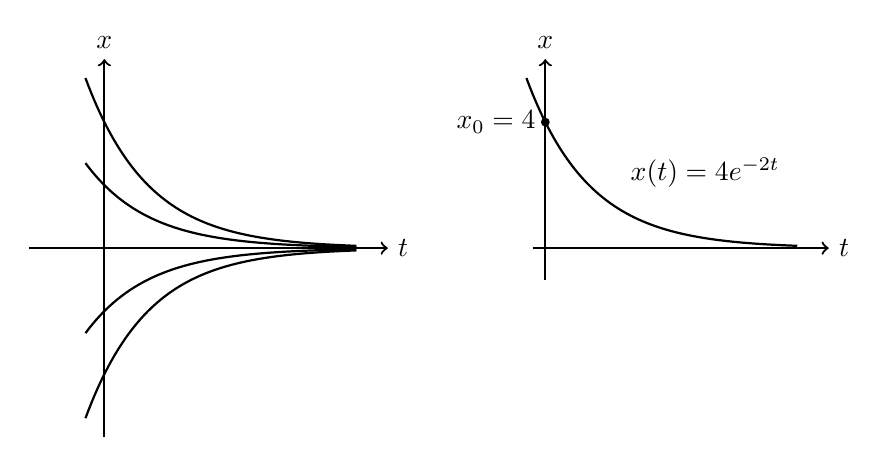
\begin{tikzpicture}[scale=0.8]
\begin{scope}
    % Axes
    \draw[->,thick] (-1.2,0) -- (4.5,0) node[right] {$t$};
    \draw[->,thick] (0,-3) -- (0,3) node[above] {$x$};

    % Curves x(t) = C e^{-t}
    \draw[thick,domain=-0.3:4,samples=100] plot (\x,{ 2*exp(-\x)});
    \draw[thick,domain=-0.3:4,samples=100] plot (\x,{ 1*exp(-\x)});
    \draw[thick,domain=-0.3:4,samples=100] plot (\x,{-1*exp(-\x)});
    \draw[thick,domain=-0.3:4,samples=100] plot (\x,{-2*exp(-\x)});
\end{scope}

\begin{scope}[xshift=7cm]
    % Axes
    \draw[->,thick] (-0.2,0) -- (4.5,0) node[right] {$t$};
    \draw[->,thick] (0,-0.5) -- (0,3) node[above] {$x$};

    % Particular solution
    \draw[thick,domain=-0.3:4,samples=100] plot (\x,{ 2*exp(-\x)});

    % Initial condition point
    \fill (0,2) circle (2pt);
    \node[left] at (0,2) {$x_0=4$};

    % Label
    \node[right] at (1.2,1.2) {$x(t)=4e^{-2t}$};
\end{scope}
\end{tikzpicture}\caption{The left figure shows a family of solutions to $x'=-2x$. The right figure shows the one particular solution with IC $x(0)=4$.}
\end{figure}

% -------------------------

\subsection{Failure of Existence} Consider the IVP
$$
\begin{dcases}
    x' = x\sqrt{t-3}\\
    x(1)=2
\end{dcases}
$$
This is a separable DE. As a review for the upcoming exam we will solve it here:
\begin{align*}
    \frac{dx}{dt} &= x \sqrt{t-3}\\
    \int \frac{dx}{x} &=  \int\sqrt{t-3}\,dt\\
    \ln|x| &=  \frac{2}{3}(t-3)^{3/2} +C\\
    x & = Ce^{2/3 (t-3)^{3/2}}
\end{align*}
Now we will apply the initial condition to solve for $C$ and...
\[
x(1)
=
Ce^{\frac{2}{3}(1-3)^{3/2}}
=
\text{undefined}.
\]
The issue is that $\sqrt{t-3}$ is only real-valued for $t\geq 3$. 

The main problem is the location of the initial condition. Since 
\[
f(t,x)=x\sqrt{t-3}
\]
is only defined for $t\geq 3$, an initial condition $(t_0,x_0)$ must lie in the region
\[
R=\{(t,x):t> 3\}
\]
shaded in the figure below. In other words, the possible initial conditions
are restricted by the domain of $f(t,x)$. Our initial condition $(1,2)$ lies outside this region, so the IVP fails existence.
\begin{figure}[H]
    \centering
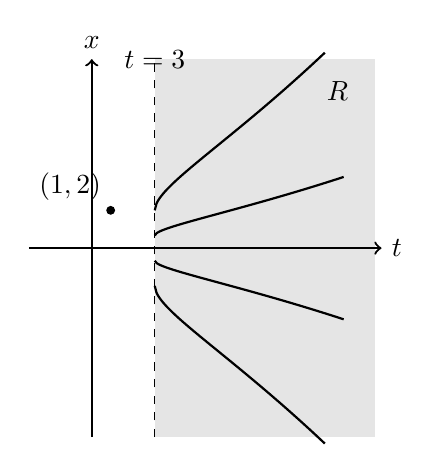
\begin{tikzpicture}[scale=0.8]
\begin{scope}
    \fill[gray!20] (1,-3) rectangle (4.5,3);
    % Axes
    \draw[->,thick] (-1,0) -- (4.6,0) node[right] {$t$};
    \draw[->,thick] (0,-3) -- (0,3) node[above] {$x$};
    % Curves x(t) = C e^{-t}
    \draw[thick,domain=1:3.7,samples=100] plot (\x,{0.6*exp(sqrt(\x-1))});
    \draw[thick,domain=1:4,samples=100] plot (\x,{0.2*exp(sqrt(\x-1))});
    \draw[thick,domain=1:4,samples=100] plot (\x,{-0.2*exp(sqrt(\x-1))});
    \draw[thick,domain=1:3.7,samples=100] plot (\x,{-0.6*exp(sqrt(\x-1))});
    % \draw[thick,domain=1:4,samples=100] plot (\x,{ 2*exp(\sqrt{\x-1})});
    % \draw[thick,domain=1:4,samples=100] plot (\x,{ 2*exp(\sqrt{\x-1})});
    % \draw[thick,domain=1:4,samples=100] plot (\x,{ 2*exp(\sqrt{\x-1})});
    \draw[dashed] (1,-3) -- (1,3) node {$t=3$};
    \fill (0.3,0.6) circle (2pt);
    \node[above left] at (0.3,0.6) {$(1,2)$};
    \node (Rlabel) at (3.9,2.5) {$R$};
\end{scope}
\end{tikzpicture}\caption{This is family of solutions to $x'=x\sqrt{t-3}$. If the IC is not in $R$ then the IVP fails existence.}
\end{figure}

% -------------------------

\subsection{Failure of Uniqueness}
Consider the IVP
$$
\begin{dcases}
    x' = 2\sqrt{x}\\
    x(0)=0
\end{dcases}
$$
This is also a separable DE. Assuming $x>0$, we can solve:
\begin{align*}
    \frac{dx}{dt} &= 2 \sqrt{x}\\
    \int \frac{dx}{\sqrt{x}} &=  \int2\,dt\\
    2\sqrt{x} &=  2t +C\\
    \sqrt{x} & = t+C\\ 
    x &= (t+C)^2
\end{align*}
Applying the initial condition gives
\[
x(0)=C^2=0,
\]
so $C=0$. Since $\sqrt{x}=t$, this solution is valid for $t\geq0$:
\[
x(t)=t^2,\qquad t\geq0.
\]
However, this is \emph{not} the only solution. The constant function $x(t)\equiv 0$ also satisfies the differential equation and the initial condition. It gets worse. If we use piecewise functions, there are infinitely many solutions. For any $a\ge 0$, the function
\[
x(t)=
\begin{cases}
0, & t\le a,\\
(t-a)^2, & t\ge a,
\end{cases}
\]
satisfies the IVP. Each solution remains at $x=0$ until time $t=a$ and then follows a
parabolic solution curve. Every one of these functions satisfies the same
initial condition $x(0)=0$. This should be quite alarming. Consider the family of functions $\mathcal{F}$. How would they appear when plotted on the $tx$-plane?

\subsection{Blow Up}

Finally, consider the IVP
\[
\begin{dcases}
    x'=x^3,\\
    x(0)=1.
\end{dcases}
\]
At a glance, this equation looks okay. The RHS $f(t,x)=x^3$ is well-defined everywhere; there are no square roots like in the previous two examples. We have solved this DE before using separation of variables. Applying the initial condition gives the unique solution
\[
x(t)=\frac{1}{\sqrt{1-2t}}.
\]
The solution exists and is unique, but its domain is limited to $t<1/2$. \textit{This function blows up!} This result is not intuitive. We expected a nice solution since the RHS $f(t,x)$ is nice. However, the interval of existence is limited to $(-\infty,1/2)$.

So what caused the blow up? This is the nature of \textit{nonlinear DEs}. Even when the right-hand side is nice, solutions can exhibit unexpected behavior. The local
regularity of $f(t,x)$ may guarantee existence and uniqueness near the
initial point, but it does not necessarily ensure a full interval of
existence.

%-------------------------------------------------------------

\section{General Existence and Uniqueness Theorem}
There are two theorems that tell us when an IVP is well-posed: one is general and the other one is specifically for linear DEs. In this section we will cover the general theorem. The general theorem applies to all first-order IVPs, but the conclusion is a bit weaker. The specific theorem in the next section applies only to linear DEs, but has a stronger conclusion.

\subsection{General Theorem}
\begin{theorem}[General Existence and Uniqueness]
Suppose $f(t,x)$ and $\partial f/\partial x$ are continuous in an open rectangle $R$ in the $tx$-plane. If $(t_0,x_0) \in R$ then the IVP
\[
x' = f(t,x),\qquad x(t_0)=x_0
\]
has a unique solution on some time interval containing $t_0$.
\end{theorem}
In plain English: "If the RHS $f(t,x)$ is nice enough at $(t_0,x_0)$, then we expect a unique solution, but we don't know if it blows up." More technically, the theorem gives us conditions that guarantee existence and uniqueness near the initial point. However, it does not tell us the maximal interval of existence.

\paragraph{Partial Derivatives} Note that $\frac{\partial }{\partial x}f(t,x)$ represents the \textbf{partial derivative} of $f$ with respect to $x$. To find the partial derivative $f_x(t,x)$, treat all $t$ terms like constants and then take the regular $x$ derivative. For example,
$$
\frac{\partial}{\partial x}(3tx^2 + (tx)^2)= 6tx +2xt^2.
$$
This is something that you should have learned (or will learn) in Calculus III.

%-------------------------------------------------------------
\subsection{Open Rectangle}

The theorem does not require $f(t,x)$ and $f_x(t,x)$ to be continuous
everywhere. We only need to find an \textbf{open rectangle} $R$ around the
initial point $(t_0,x_0)$ where both functions are continuous. An open rectangle in the $tx$-plane has the form
\[
R=\{(t,x):a<t<b,\;c<x<d\}
  =(a,b)\times(c,d).
\]
The word \textbf{open} means that the boundary of the rectangle is not
included, which we indicate with dashed lines. The important condition is that the initial point must be \textit{inside}
the rectangle:
\[
(t_0,x_0)\in R.
\]
If $f$ and $f_x$ are continuous throughout $R$, then the theorem guarantees
a unique solution on some interval containing $t_0$.

\begin{figure}[H]
    \centering
\begin{tikzpicture}[scale=0.75]
    % axes
    \draw[->,thick] (0,0) -- (7.2,0) node[right] {$t$};
    \draw[->,thick] (0,0) -- (0,5.2) node[above] {$x$};

    % key x-levels
    \def\yC{1.2}
    \def\yX{2.7}
    \def\yD{4.2}
    % key t-locations
    \def\tA{1.1}
    \def\tAl{2.6}
    \def\t0{4.2}
    \def\tBe{5.6}
    \def\tB{6.8}
    % y-axis labels c, x0, d
    \node[left] at (0,\yC) {$c$};
    \node[left] at (0,\yX) {$x_0$};
    \node[left] at (0,\yD) {$d$};

    % x-axis labels a, alpha, t0, beta, b
    \node[below] at (\tA,0) {$a$};
    % \node[below] at (\tAl,0) {$\alpha$};
    \node[below] at (\t0,0) {$t_0$};
    % \node[below] at (\tBe,0) {$\beta$};
    \node[below] at (\tB,0) {$b$};

    % dashed rectangle: [alpha,beta] x [c,d]
    \draw[dashed,thick] (\tA,\yC) rectangle (\tB,\yD);

    % dashed lines to (t0,x0)
    \draw[dashed] (0,\yX) -- (\t0,\yX);
    \draw[dashed] (\t0,0) -- (\t0,\yX);

    % point (t0,x0)
    \fill (\t0,\yX) circle (1.6pt);
    \node[right] at (\t0+0.15,\yX+0.15) {$(t_0,x_0)$};
    \draw[thick]
        plot[smooth,tension=0.8]
        coordinates {(\tAl+0.65,\yC+1.0) (\t0,\yX)  (\tBe-0.55,\yD-0.55)};
\end{tikzpicture}
    \caption{Draw the open rectangle $R=(a,b)\times(c,d)$ with a dashed boundary.}
\end{figure}

\subsection{Using the Theorem}
To apply the theorem:
\begin{enumerate}
    \item Compute $f_x(t,x)$.
    \item Determine where both $f(t,x)$ and $f_x(t,x)$ are continuous.
    \item Check whether an open rectangle $R$ containing $(t_0,x_0)$ can
    fit entirely inside this region.
\end{enumerate}


\begin{example}[1]{

 Explain why the IVP $x'=2\sqrt{x}$ with $x(0)=0$ fails uniqueness.

}
 
 The RHS $f(t,x)=2\sqrt{x}$ is continuous wherever $x\ge0$, so it is continuous at $x=0$ and above. But the derivative $f_x(t,x) = \frac{1}{\sqrt{x}}$ is not defined at $x=0$, so the rectangle is 
    $$
    R = (-\infty,\infty)\times (0,\infty).
    $$
    In order for this IVP to have existence and uniqueness, we need the initial point $(t_0,x_0)$ to be \emph{strictly inside} the box, but $(0,0)$ right on the boundary of $R$. The theorem cannot guarantee  

\begin{figure}[H]
\centering
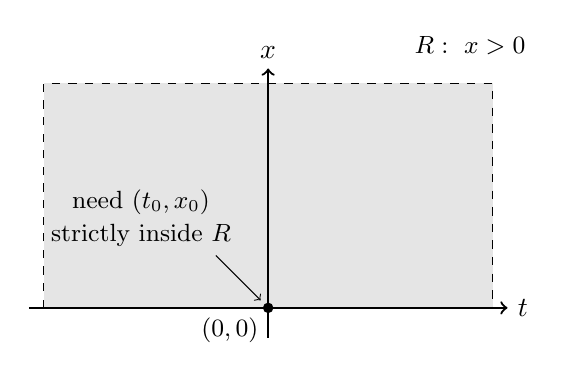
\begin{tikzpicture}[scale=0.95]
    % shade admissible rectangle R = (-inf,inf) x (0,inf) in the viewing window
    \fill[gray!20] (-3,0) rectangle (3,3);
    \draw[dashed] (-3,0) rectangle (3,3);
    % axes
    \draw[->,thick] (-3.2,0) -- (3.2,0) node[right] {$t$};
    \draw[->,thick] (0,-0.4) -- (0,3.2) node[above] {$x$};

    % boundary x=0 (excluded because f_x not defined there)
    % \draw[dashed,thick] (-4,0) -- (4,0);
    % \node[right] at (4,0) {\small $x=0$ (excluded for $f_x$)};

    % label region
    \node at (2.7,3.5) {\small $R:\ x>0$};

    % show the "bad" initial point (0,0) on the boundary
    \fill (0,0) circle (2pt);
    \node[below left] at (0,0) {\small $(0,0)$};

    % % show an allowed initial point (t0,x0) strictly inside
    % \fill (1.8,1.6) circle (2pt);
    % \node[right] at (1.8,1.6) {\small $(t_0,x_0)$ with $x_0>0$};

    % small note about why this matters
    \node[align=center] at (-1.7,1.2) {\small need $(t_0,x_0)$\\ \small strictly inside $R$};
    \draw[->] (-0.7,0.7) --(-0.1,0.1);
\end{tikzpicture}

\end{figure}

    
\end{example}

    

\begin{example}[2]{
    
Consider the IVP
$$
x' = \ln(x-1)+\sqrt{t^2-4}, \qquad x(t_0)=x_0.
$$
For which initial points $(t_0,x_0)$ are we assured that a unique solution exists? Sketch the region of all acceptable initial conditions in the $tx$-plane.
}

First, let
\[
f(t,x)=\ln(x-1)+\sqrt{t^2-4}.
\]
Its partial derivative with respect to $x$ is
\[
f_x(t,x)=\frac{1}{x-1}.
\]
This does not introduce any additional restrictions on the domain.

For $f(t,x)$ to be defined, we need
\[
x-1>0 \quad \text{and} \quad 
t^2-4\geq0.
\]
Thus, both $f$ and $f_x$ are continuous in the region
\[
x>1,\qquad |t|\geq2.
\]

However, the General Existence and Uniqueness Theorem requires the initial
point $(t_0,x_0)$ to lie inside an \emph{open rectangle} on which both
$f$ and $f_x$ are continuous.

Therefore, we cannot choose an initial point on the boundaries $t=\pm2$.
There is no open rectangle around such a point that remains inside the
domain of $f$.

Hence, the theorem guarantees a unique solution whenever
\[
x_0>1,\qquad |t_0|>2.
\]

Equivalently, the acceptable initial conditions form the region
\[
\{(t,x):x>1,\ t<-2\}
\cup
\{(t,x):x>1,\ t>2\}.
\]
\begin{figure}[H]
\centering
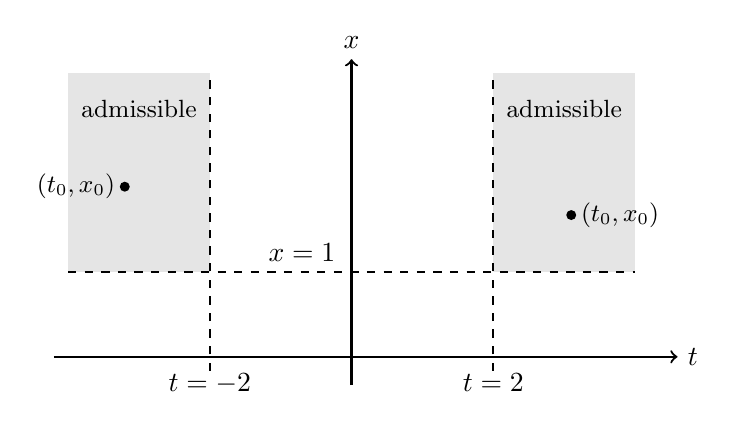
\begin{tikzpicture}[scale=0.90]
    % axes
    \draw[->,thick] (-4.2,0) -- (4.6,0) node[right] {$t$};
    \draw[->,thick] (0,-0.4) -- (0,4.2) node[above] {$x$};

    % shade admissible initial conditions:
    % x>1 and t<-2 or t>2
    \fill[gray!20] (-4,1.2) rectangle (-2,4.0);
    \fill[gray!20] ( 2,1.2) rectangle ( 4,4.0);

    % excluded boundaries
    \draw[dashed,thick] (-4,1.2) -- (4,1.2);
    \draw[dashed,thick] (-2,-0.2) -- (-2,4.0);
    \draw[dashed,thick] ( 2,-0.2) -- ( 2,4.0);

    % boundary labels
    \node[above] at (-0.7,1.2) {$x=1$};
    \node[below] at (-2,-.1) {$t=-2$};
    \node[below] at ( 2,-.1) {$t=2$};

    % region labels
    \node at (-3.0,3.5) {\small admissible};
    \node at ( 3.0,3.5) {\small admissible};

    % sample admissible initial points
    \fill (-3.2,2.4) circle (2pt);
    \node[left] at (-3.2,2.4) {\small $(t_0,x_0)$};

    \fill (3.1,2.0) circle (2pt);
    \node[right] at (3.1,2.0) {\small $(t_0,x_0)$};

\end{tikzpicture}

\end{figure}
\end{example}


\subsection{Nonlinear DEs}

There is an important limitation to the general theorem. Even if $f(t,x)$
and $f_x(t,x)$ are smooth everywhere, the theorem only guarantees a unique
solution on \textit{some} interval containing $t_0$. It does not guarantee
that the solution exists for all time.

This is one of the difficulties with \textbf{nonlinear DEs}. Solutions can
exhibit unexpected behavior, such as blowing up in finite time, even when
the differential equation itself is perfectly smooth. Thus, the regularity
of $f(t,x)$ tells us a great deal about \textit{local} existence and
uniqueness, but much less about the \textit{global} behavior of the solution. In the next section, we will see that linear DEs behave much more nicely.

%-------------------------------------------------------------
\section{Global Existence Theorem}
If the DE is \textit{linear} $x' + p(t)x = q(t)$ we may use a stronger version of the existence theorem.  

\subsection{Theorem Statement}
\begin{theorem}[Existence and Uniqueness for Linear DEs]
Consider the linear initial value problem
\[
x' + p(t)x = q(t), \qquad x(t_0)=x_0.
\]
If $p(t)$ and $q(t)$ are continuous on an open interval $I$ containing
$t_0$, then the IVP has a unique solution defined on the entire interval
$I$.
\end{theorem}
This theorem is more useful for a couple of reasons. First, it is not
necessary to take any derivatives. Second, the theorem gives us much more
information about the interval of existence. To find the largest interval guaranteed by the theorem, find where both
$p(t)$ and $q(t)$ are continuous. Then choose the largest open interval
containing $t_0$. You do not have to deal with rectangles, but you do have
to keep track of where the initial condition resides.


\subsection{Using the Theorem}

For a linear IVP
\[
x'+p(t)x=q(t),\qquad x(t_0)=x_0,
\]
we can determine the interval of existence without actually solving the DE.

\begin{enumerate}
    \item Find where both $p(t)$ and $q(t)$ are continuous.

    \item Express the region of continuity as unions of \textit{open subintervals}.

    \item The interval of existence is the subinterval that contains the initial time $t_0$.
\end{enumerate}
The theorem guarantees that the IVP has a unique solution throughout this
entire interval. The initial value $x_0$ does not affect the interval. What matters is the
initial time $t_0$ and where the coefficient functions $p(t)$ and $q(t)$
are continuous.
\begin{example}[3]{
State the interval of existence of the following IVP
\[
x' + \frac{1}{t-2}x = \sin t,\qquad x(0)=1.
\]
}
Notice that this is a liner DE with
\[
p(t)=\frac{1}{t-2},\qquad q(t)=\sin t.
\]
The function $q(t)$ is continuous everywhere, but $p(t)$ is not continuous at $t=2$, so their common domain is $(-\infty,2,)\cup(2,\infty)$. 
Since $t_0=0$, the largest open interval containing $0$ that avoids $t=2$ is
\[
\boxed{(-\infty,2).}
\]
\end{example}

\begin{example}[4]{    
State the interval of existence of the following IVP
\[
x' + \frac{1}{t^2-1}x = e^t,\qquad x(2)=0.
\]
}
The coefficient
\[
p(t)=\frac{1}{t^2-1}
\]
has singularities at $t=\pm 1$. Therefore, the domain consists of the union of three subintervals $(-\infty,-1)\cup (-1,1)\cup(1,\infty)$. 
Since $t_0=2 \in(1,\infty)$, the interval of existence is
\[
\boxed{(1,\infty).}
\]
\end{example}

\subsection{Behavior at the Endpoints}

There is one final subtlety about the interval of existence. A solution must
be defined and finite at every point \textit{inside} the interval, but it
does not need to remain bounded as it approaches an endpoint. For example, suppose the theorem guarantees a unique solution on
\[
I=(-\infty,2).
\]
It is perfectly possible that
\[
\lim_{t\to2^-}x(t)=\infty.
\]
This is not a failure of the theorem. The endpoint $t=2$ is not contained
in the open interval $I$, so the theorem makes no claim about what happens
there. 

% \begin{example}[]{
% Consider
% \[
% x' + (\ln t)x = t,\qquad x(1)=3.
% \]
% }
% Here $p(t)=\ln t$ is only defined for $t>0$.
% Thus the largest open interval containing $t_0=1$ is
% \[
% \boxed{(0,\infty).}
% \]
% \end{example}

% \section{Table}
% Here is a table that summarizes the two theorems.
% \begin{table}[H]
% \centering
% \renewcommand{\arraystretch}{1.35}
% \begin{tabular}{|p{4.2cm}|p{5.1cm}|p{5.1cm}|}
% \hline

% & \textbf{General IVP Theorem} 
% & \textbf{Linear IVP Theorem} \\ \hline

% Type of equation 
% & $x' = f(t,x)$ 
% &  $x' + p(t)x = q(t)$ \\ \hline

% Conditions on RHS 
% & $f(t,x)$ and $\partial f/\partial x$ continuous 
% & $p(t)$ and $q(t)$ continuous \\ \hline

% What is guaranteed? 
% & Existence and uniqueness 
% & Existence, uniqueness, and interval of existence \\ \hline

% Interval of existence 
% & Some (unknown) interval around $t_0$ 
% & Entire interval where $p(t),q(t)$ are continuous \\ \hline

% Does it prevent blow-up? 
% & No 
% & Yes (within the interval) \\ \hline

% Can the solution fail later? 
% & Yes 
% & Only at coefficient singularities \\ \hline

% Typical conclusion 
% & ``A unique solution exists locally somewhere in this region'' 
% & ``A unique solution exists on this whole interval'' \\ \hline

% How to find the interval 
% & Not specified by the theorem 
% & Find the domain of $p(t)$ and $q(t)$ \\ \hline

% Common failure modes 
% & Non-uniqueness, blow-up, short lifespan 
% & Coefficient singularities only \\ \hline

% \end{tabular}

% \end{table}


\end{document}
